\documentclass[10pt]{article}

\usepackage[latin1]{inputenc}
\usepackage{amsmath, amssymb, amsfonts, amsthm}
\usepackage{upgreek}
\usepackage{amsthm}
\usepackage{fullpage}
\usepackage{graphicx}
\usepackage{cancel}
\usepackage{subfigure}
\usepackage{mathrsfs}
\usepackage{outlines}
\usepackage[font={sf,it}, labelfont={sf,bf}, labelsep=space, belowskip=5pt]{caption}
\usepackage{hyperref}
% \usepackage{minted}
\usepackage{enumerate}
\usepackage{titling}

\usepackage{fancyhdr}
\usepackage[title]{appendix}

\DeclareMathOperator{\sgn}{sgn}

\pagestyle{fancy}
\headheight 24pt
\headsep    12pt
\lhead{Objectives for Pattern Parameter Optimization}
\rhead{\today}
\fancyfoot[C]{} % hide the default page number at the bottom
\lfoot{}
\rfoot{\thepage}
\renewcommand{\headrulewidth}{0.4pt}
\renewcommand\footrulewidth{0.4pt}
\providecommand{\abs}[1]{\lvert#1\rvert}
\providecommand{\norm}[1]{\lVert#1\rVert}
\providecommand{\dx}{\, \mathrm{d}x}
\providecommand{\dA}{\, \mathrm{d}A}
% \providecommand{\vint}[2]{\int_{#1} \! #2 \, \mathrm{d}x}
% \providecommand{\sint}[2]{\int_{\partial #1} \! #2 \, \mathrm{d}A}
\renewcommand{\div}{\nabla \cdot}
\providecommand{\shape}{\Omega(p)}
\providecommand{\mesh}{\mathcal{M}}
\providecommand{\boundary}{\partial \shape}
\providecommand{\vint}[1]{\int_{\shape} \! #1 \, \mathrm{d}x}
\providecommand{\sint}[1]{\int_{\boundary} \! #1 \, \mathrm{d}A}
\providecommand{\pder}[2]{\frac{\partial #1}{\partial #2}}
\providecommand{\tder}[2]{\frac{\mathrm{d} #1}{\mathrm{d} #2}}
\providecommand{\evalat}[2]{\left.#1\right|_{#2}}
\newcommand{\defeq}{\vcentcolon=}
\newtheorem{lemma}{Lemma}

\makeatletter
\usepackage{mathtools}
\newcases{mycases}{\quad}{%
  \hfil$\m@th\displaystyle{##}$}{$\m@th\displaystyle{##}$\hfil}{\lbrace}{.}
\makeatother

\setlength{\droptitle}{-80pt}
\title{Objectives for Pattern Parameter Optimization}
\author{Julian Panetta}

% BEGIN DOCUMENT
\begin{document}
\maketitle

We start by seeking an objective function to fit a
particular (flattened) elasticity tensor, $C$, to a target tensor, $C^*$.
We first show the na\"ive objective penalizing (squared) Frobenius norm
distance, $$J_C = ||C - C^*||^2_F$$ is poorly behaved and then propose a more
physically motivated objective function: Frobenius norm distance of the
flattened compliance tensors. Finally, we suggest various improvements over this objective,
including reformulating the pattern optimization as a direct minimization of
the global displacement-fitting objective,
\begin{equation}
\begin{aligned}
\label{eqn:main_objective}
J_\text{u} = \int_{\Gamma} \norm{P(u - u^*)}^2 \dA \quad \text{s.t.} \\
-\nabla \cdot [C(x) : \epsilon(u)] = f \text{ in } \Omega \\
\hat{n} \cdot [C(x) : \epsilon(u)] = g \text{ on } \Omega,
\end{aligned}
\end{equation}
that is used for material optimization. Here $\Gamma \subseteq \partial \Omega$
is the portion of the boundary where target displacements $u^*$ are specified,
and $P$ is a matrix that projects out unspecified components of $u^*$ (e.g., if
we only want to specify the $y$ coordinate of the target displacement).

Throughout this discussion, it is important to keep in mind that this is the
over-all goal of our pipeline: to achieve the target displacements, $u^*$.

\section{Problems with $J_C$}
We examine objective $J_C$ in a simplified 2D setting where both $C$ and
$C^*$ are isotropic (functions of Young's modulus $E$ and Poisson ratio $\nu$):

$$
J_C(E, \nu) =
    \left\lVert
    E
    \left(
    \begin{array}{ccc}
     \frac{1}{1-\nu ^2} & \frac{\nu }{1-\nu ^2} & 0 \\
     \frac{\nu }{1-\nu ^2} & \frac{1}{1-\nu ^2} & 0 \\
     0 & 0 & \frac{1}{2 \nu +2} \\
    \end{array}
    \right) -
    E^*
    \left(
    \begin{array}{ccc}
     \frac{1}{1-{\nu^*} ^2} & \frac{{\nu^*} }{1-{\nu^*} ^2} & 0 \\
     \frac{{\nu^*} }{1-{\nu^*} ^2} & \frac{1}{1-{\nu^*} ^2} & 0 \\
     0 & 0 & \frac{1}{2 {\nu^*} +2} \\
    \end{array}
    \right)
    \right\rVert^2_F
$$

There are two drawbacks with this objective:

\begin{enumerate}
\item Deviations of Young's modulus and Poisson ratios are not penalized in a
      physically meaningful way.
\item Poisson ratio and Young's modulus effects are not neatly separated.
\end{enumerate}

\subsection{Nonphysical penalty on deviations}
First, consider the simplified case, $\nu = \nu^*$. Then, the Frobenius
norm objective reduces to:
$$
J_C(E, \nu) = f(\nu^*) (E - E^*)^2 \quad \text{where } f(\nu) = \frac{9 {\nu} ^2-2 {\nu} +9}{4 \left({\nu} ^2-1\right)^2}
$$

Thus, the penalty is quadratic in $E - E^*$, with a coefficient that blows up at $\nu = \nu^* = \pm 1$:
\\
\begin{minipage}{\linewidth}
    \centering
    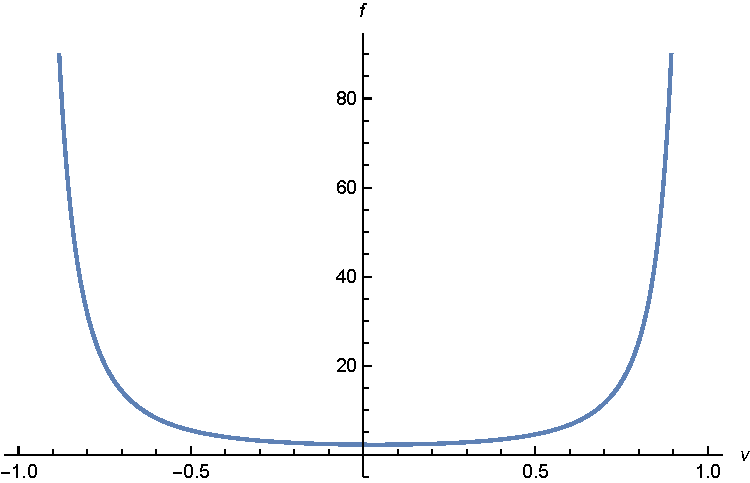
\includegraphics[width=.5\textwidth]{quadraticCoefficient.pdf}
\end{minipage}

A penalty proportional to squared absolute distance $(E - E^*)^2$ is bad for
two obvious reasons:

\begin{enumerate}
    \item An particular absolute difference from $E^* = 1$ is much worse (from a
        displacements perspective) than the same absolute difference from $E^* =
        100$, suggesting that there could be weighting problems in the
        anisotropic case with differing $E_x^*$ and $E_y^*$. 
\item More seriously, consider $E^* = 1$ and compare the behavior with $E = .5$
    and $E = 1.5$ (both with the same relative and absolute difference from
    $E^*$). The Frobenius norm objective assigns the same penalty to both, but
    the former will deform twice as much with a particular load (a $100\%$
    displacement difference), while the latter deforms $2/3$ as much (only a $33\%$
    difference). We clearly want our objective to penalize the former more.
\end{enumerate}

Now, consider the case $E = E^*$, where the objective reduces to:
$$
J_C(E, \nu) = j(\nu) E^2 \quad \text{where }
j = 
    2 \left(\frac{1}{1-\nu ^2}-\frac{1}{1-{\nu^*}^2}\right)^2+2
    \left(\frac{\nu }{1-\nu ^2}-\frac{{\nu^*}}{1-{\nu^*}^2}\right)^2+\left(\frac{1}{2 \nu +2}-\frac{1}{2 {\nu^*}+2}\right)^2
$$

$J_C(1, \nu)$ is plotted below with various target Poisson ratios, $\nu^*$ in
the range $-0.4$ to $0.8$, with a zoomed out view on the right.
\\
\begin{minipage}{\linewidth}
    \centering
    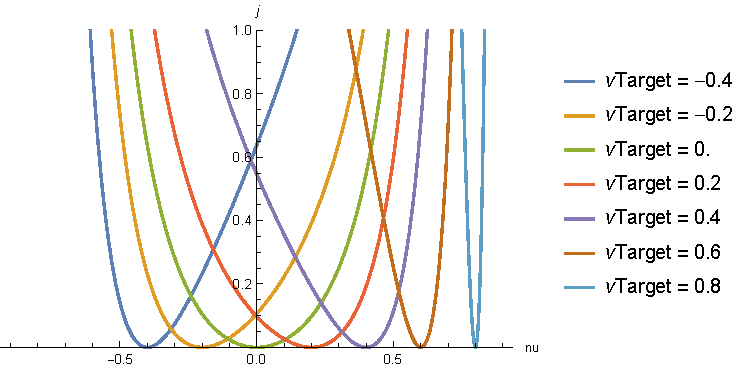
\includegraphics[width=.45\textwidth]{vPlot.pdf}
    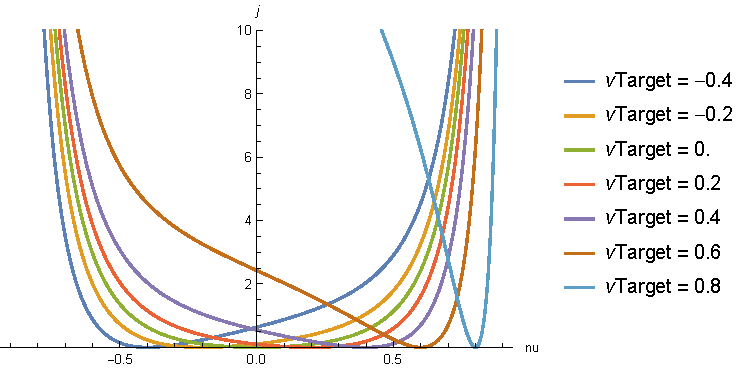
\includegraphics[width=.45\textwidth]{vPlotZoomOut.pdf}
\end{minipage}
Small deviations from $\nu^*$ are penalized much more severely at higher values
of $\left|\nu^*\right|$, which is the opposite of what we want from a
relative-displacement-error perspective.

\subsection{Interplay of $E$ and $\nu$}
When either $E$ or $\nu$ differs from its target value, the
elasticity-tensor-based objective, $J_C$, does a poor job of fitting the other
parameter.

For example, consider a target isotropic tensor $E^* = 5, \nu^* = 0.3$. When
$\nu$ deviates from $\nu^*$, the optimal $E$ according to $J_C$ drifts away from
$E^*$. As $\nu^*$ becomes larger, this effect becomes more pronounced:
\\
\begin{minipage}{\linewidth}
    \centering
    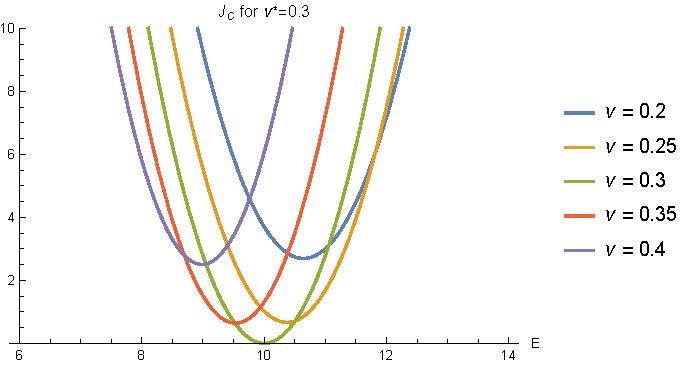
\includegraphics[width=.45\textwidth]{interplayE.pdf}
    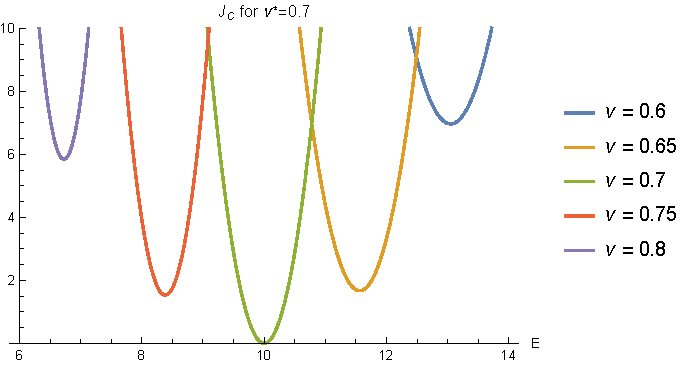
\includegraphics[width=.45\textwidth]{interplayELargeNu.pdf}
\end{minipage}
In practice, this has caused bad Young's moduli to be chosen by the lookup
table projection when Poisson ratio cannot be matched closely.

\section{Better objectives}
We consider better-behaved objectives than $J_C$, first ignoring the greater goal of minimizing $J_u$.

\subsection{$J_S$: Compliance-based, ``absolute displacements'' objective}
Most of the problems mentioned above can be fixed by instead penalizing the
Frobenius norm distance of the (flattened) compliance tensors $S$ and $S^*$:
$$
    J_S = ||S - S^*||^2_F.
$$

In the 2D orthotropic case using the flattening conventions from the tensor
flattening writeup, this can be written as:
\begin{equation}
    \label{eqn:JS}
J_S(E_x, E_y, \nu_{yx}, \mu) = 
\left(\frac{1}{E_x} - \frac{1}{E_x^*}\right)^2 +
\left(\frac{1}{E_y} - \frac{1}{E_y^*}\right)^2 +
2 \left(\frac{\nu_{yx}}{E_y} - \frac{\nu_{yx}^*}{E_y^*}\right)^2 +
\frac{1}{16} \left(\frac{1}{\mu} - \frac{1}{\mu^*}\right)^2
\end{equation}
Each term has a nice physical interpretation: consider two squares with edge
length $l$, one filled with material $(E_x, E_y, \nu_{yx}, \mu)$ and the other
with target material $(E_x^*, E_y^*, \nu_{yx}^*, \mu^*)$. Each term of $J_S$
measures how the two squares' displacements differ when probed with a particular
load.

For example, consider a vertical load that stretches the squares, causing a
constant strain and stress displacement:
\\
\begin{minipage}{\linewidth}
    \centering
    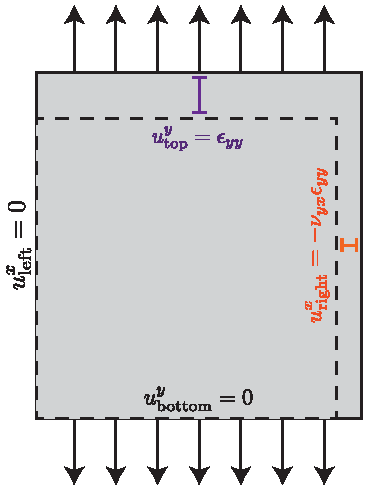
\includegraphics[width=.35\textwidth]{y_load.pdf}
\end{minipage}
Choosing coordinates so that the bottom and left edges do not displace (or
applying Dirichlet conditions), the displacements of the squares' tops are:
$$
u^y_\text{top} = l \epsilon_{yy} = \frac{l \sigma_{yy}}{E_y}, \quad
{u^y_\text{top}}^* = l \epsilon^*_{yy} = \frac{l \sigma_{yy}}{E^*_y},
$$
and the displacements of their right edges are:
$$
u^x_\text{right} = l \epsilon_{xx} = -l \nu_{yx} \epsilon_{yy} = -\frac{l \sigma_{yy} \nu_{yx}}{E_y}, \quad
{u^x_\text{right}}^* = l \epsilon^*_{xx} = l \nu_{yx}^* \epsilon^*_{yy} = -\frac{l \sigma_{yy} \nu_{yx}^*}{E^*_y}.
$$
Choosing a vertical load such that $\sigma_{yy} = \frac{1}{l}$ (i.e. total force 1N),
$$
u^y_\text{top} = \frac{1}{E_y}, \quad {u^y_\text{top}}^* = \frac{1}{E^*_y}, \quad
u^x_\text{right} = -\frac{\nu_{yx}}{E_y}, \quad {u^x_\text{right}}^* = -\frac{\nu_{yx}^*}{E^*_y},
$$
and the second and third terms of $J_S$ in (\ref{eqn:JS}) clearly penalize the
(squared) difference in
resulting top and left displacements. Similarly, the first and third terms can be interpreted as
penalizing the (squared) difference in left and top displacements under a
horizontal load causing $\sigma_{xx} = \frac{1}{l}$.

Now, consider applying a constant-strain shearing displacement:
\\
\begin{minipage}{\linewidth}
    \centering
    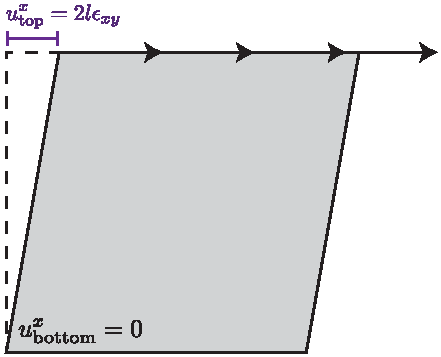
\includegraphics[width=.35\textwidth]{shear_load.pdf}
\end{minipage}
This is done by prescribing normal traction $(\sigma_{xy}, 0)^T$ at the top
face and a $u = 0$ Dirichlet boundary condition on the bottom face. In this case, 
$$
u^x_\text{top} = 2 l \epsilon_{xy} = 2 l \frac{\sigma_{xy}}{2 \mu} = \frac{l \sigma_{xy}}{\mu},\quad
{u^x_\text{top}}^* = \frac{l \sigma_{xy}}{\mu^*}.
$$
Choosing $\sigma_{xy} = \frac{1}{l}$ (total force 1N) gives $x$ displacements
of the top whose squared difference is measured by the fourth term in (\ref{eqn:JS}).

Thus, minimizing $J_S$ can be viewed as a multi-objective optimization---trying
to simultaneously fit five 1N displacements---that has been ``linearly
scalarized'' with particular weights (the third term in (\ref{eqn:JS}) actually
penalizes two different displacement quantities that equal). This scalarization
is guaranteed to give us a Pareto optimal solution to the multi-objective
problem, but not necessarily the Pareto optimum we want. For example, the shear
term is probably weighted much less than it should be. Ideally we would
choose weights based on how sensitive the over-all objective
(\ref{eqn:main_objective}) is to an error in each of the sub-objectives.

\subsection{Full vs. flattened tensor norms}
There is a question whether we should be using the matrix Frobenius norm on the
flattened tensors, as done in (\ref{eqn:JS}), or the full rank four tensor
Frobenius norm. As shown in the Tensor Flattening writeup, the difference is in
the scaling of the shear term only. The symmetric rank 4 tensor version is:
\begin{equation}
    \label{eqn:JS4}
J_{S4}(E_x, E_y, \nu_{yx}, \mu) = 
\left(\frac{1}{E_x} - \frac{1}{E_x^*}\right)^2 +
\left(\frac{1}{E_y} - \frac{1}{E_y^*}\right)^2 +
2 \left(\frac{\nu_{yx}}{E_y} - \frac{\nu_{yx}^*}{E_y^*}\right)^2 +
\frac{1}{4} \left(\frac{1}{\mu} - \frac{1}{\mu^*}\right)^2
\end{equation}

But since the rank 4 tensor implementing the strain to stress mapping is not
unique, this is not the only possible Frobenius norm. Furthermore, we could have
flattened in a different way when formulating (\ref{eqn:JS}). For example, we
could instead use the matrix mapping flattened stress to engineering strain
(this matrix is no longer symmetric in general, and its entries are no longer in
direct correspondence with the compliance tensor entries):
$$
S' = \begin{pmatrix}
    \frac{1}{E_x} & -\frac{\nu_{yx}}{E_y} & 0 \\
    -\frac{\nu_{yx}}{E_y} & \frac{1}{E_y}  & 0 \\
    0 & 0 & \frac{1}{\mu}
\end{pmatrix},
$$
which would give the objective
\begin{equation}
    \label{eqn:JS'}
J_{S'}(E_x, E_y, \nu_{yx}, \mu) = 
\left(\frac{1}{E_x} - \frac{1}{E_x^*}\right)^2 +
\left(\frac{1}{E_y} - \frac{1}{E_y^*}\right)^2 +
2 \left(\frac{\nu_{yx}}{E_y} - \frac{\nu_{yx}^*}{E_y^*}\right)^2 +
\left(\frac{1}{\mu} - \frac{1}{\mu^*}\right)^2.
\end{equation}

Carefully choosing one from the many possible ``Frobenius norms'' may not be
worthwhile; the following objectives propose different weightings from those in
(\ref{eqn:JS}) anyway.

\subsection{Relative displacements objective function}
We can weight the terms in another way that makes the quantities dimensionless
and neatly separates the Young's modulus and Poisson ratio parameters. This is
desirable in circumstances where the relative error of the displacements matters
as opposed to the absolute error. For example, if one cares about fitting
accurately small (nonzero!) Poisson ratios, a relative error measurement will
prevent the Young's moduli terms of (\ref{eqn:JS}) from dominating.

Dividing each term in (\ref{eqn:JS}) by the corresponding target displacement
quantity, we arrive at:
$$
J_{rel} = \left(\frac{E_x^*}{E_x} - 1 \right)^2 + \left(\frac{E_y^*}{E_y} - 1 \right)^2
    + 2 \left(\frac{\nu_{yx}}{\nu_{yx}^*} - 1 \right)^2
    + \left(\frac{\mu^*}{\mu} - 1 \right)^2
$$
Now the objective is also independent of the ``total force'' of each scenario,
which before was arbitrarily set to 1N.
Of course, if absolute displacement under equal-force loading scenarios is what we
care about (or if $\nu_{xy}^* = 0$), we're better off using the plain $J_S$.

\section{Global displacement-aware objectives}
We now attempt to formulate an objective that uses more information from the
material optimization stage than just the target tensors. The full solution
from the material optimization stage offers two extra pieces of information:

\begin{enumerate}[(a)]
    \item The load on the cell under the ``optimal'' material field we're trying to fit.
          \label{it:load}
    \item The sensitivity of the over-all objective, (\ref{eqn:main_objective}),
          to each parameter.
          \label{it:sensitivity}
\end{enumerate}

Using (\ref{it:load}), we no longer need to consider the same arbitrary five 1N
load scenarios that $J_S$ does---we can focus on the particular load we expect
the cell to bear. However, exactly fitting the strain under this load might not
be the most important goal; some strain components are likely unimportant to
the global displacement objective. Section \ref{sec:strain_fit} elaborates on this option.

Using (\ref{it:sensitivity}), we have two options: we could use the sensitivity
information to weight each term of $J_S$, or we could discard $J_S$ entirely
and use chain rule to directly optimize $J_u$ (treating
the material optimization stage + pattern lookup as giving an initial guess for
pattern/shape optimization of $J_u$). Sections \ref{sec:sensitivity_weight}
and \ref{sec:chain_rule} elaborate on these two options.

\subsection{Strain-fitting objective}
\label{sec:strain_fit}
Using the constant cell strain and stress from the material optimization stage,
$\epsilon^*$ and $\sigma$, we can minimize:
$$
J_\text{strain} = \norm{\epsilon - \epsilon^*}^2_F = \norm{S \sigma - S^* \sigma}_F^2
$$
Notice how this is essentially identical to the local step of the local-global
material optimization algorithm. In fact, we could run a few iterations of the
local-global material optimization algorithm, then project the material tensors into
pattern parameter space with the look-up table (using $J_\text{strain}$) and
run more local-global iterations in pattern parameter space  (using the shape
derivative of $J_\text{strain}$ and taking $\epsilon^*$ from a Dirichlet
solve). This merging of pattern and material optimization is similar in spirit to
the approach in Section \ref{sec:chain_rule}.

\subsection{Sensitivity-weighted objective}
\label{sec:sensitivity_weight}
Unfortunately, using the above objective doesn't solve one problem we've seen in
practice. Some parameter (say, Poisson ratio), may be unimportant in
achieving a particular target deformation. All objectives discussed so far consider all
parameters (or in the case of $J_\text{strain}$, all strain components)
as equally important. If the objective favors closely fitting an unimportant
parameter at the expense of a more important parameter, the pattern optimizer
likely will choose a suboptimal elasticity tensor with respect to the global
displacement objective, $J_u$; we need some way of weighting the terms in $J_S$ so
that we choose good point on its Pareto curve.

One possible way to do this is to consider the analytic derivative of $J_u$
with respect to $\frac{1}{Ex}$, $\frac{\nu_{yx}}{Ey}$, $\dots$ computed via the
adjoint method. The magnitude of each derivative evaluated at $C^*$ gives a sense
of how important it is to fit the corresponding terms of $J_S$ and could be used as a
weight. Of course, if the $C^*$ found by material optimization happens to be
perfectly optimal (unlikely), these derivatives would all be zero, and one could
instead evaluate at a nearby, perturbed point in material parameter space.

\subsection{Global-displacement objective (i.e. massive chain rule)}
\label{sec:chain_rule}
Of course, it's possible to use more than just the magnitude of the derivatives
of $J_u$; since we can compute derivatives of $J_u$ with respect to
$\frac{1}{Ex}$, $\frac{\nu_{yx}}{Ey}$, $\dots$, and we can compute shape
derivatives of these quantities, we can compute the full shape derivative of
$J_u$ and thus the derivative of $J_u$ with respect to each pattern parameter.

This means that we would use the same energy for pattern optimization as material
optimization, and the two stages (material optimization then pattern parameter
optimization) could be interpreted as two levels of a multi-resolution optimization
(an optimization at the macroscopic-scale followed by a projection to and an
optimization at the microscopic scale).

\end{document}
